\documentclass[a4paper, 12pt, oneside]{report}

\usepackage{preamble}

\begin{document}

\noindent \textbf{Práctica 7} \hfill \textbf{David López del Pino}

\hfill

En esta práctica se implementan varios esquemas en diferencias finitas implícitos para la ecuación del calor. 

Si llamamos $N$ al número de puntos de la discretización en espacio, habrá que resolver un sistema lineal de $N$ ecuaciones y $N$ incógnitas. Primero consideramos condiciones de contorno de Dirichlet, $D_L$ a la izquierda y $D_R$ a la derecha. Tenemos entonces $N-2$ ecuaciones y $N-2$ incógnitas, pues $u_0^{n+1}$ y $u_{N-1}^{n+1}$ son conocidos. 

El esquema a considerar en el primer apartado de la práctica es, como vimos en clase, $AU^{n+1} = B^n$, es decir,
\[\left(\begin{array}{ccccc}
    1+2s & -s & \cdots & 0 & 0 \\
    -s & 1+2s & \cdots & 0 & 0 \\
    \vdots & \vdots & \ddots & \vdots & \vdots \\
    0 & 0 & \cdots & 1+2s & -s \\
    0 & 0 & \cdots & -s & 1+2s
\end{array}\right)\left(\begin{array}{c}
    u_1^{n+1} \\
    u_2^{n+1} \\
    \vdots \\
    u_{N-3}^{n+1} \\
    u_{N-2}^{n+1}
\end{array}\right) = \left(\begin{array}{c}
    u_1^n + sD_L(t_{n+1}) \\
    u_2^n \\
    \vdots \\
    u_{N-3}^n \\
    u_{N-2}^n + sD_R(t_{n+1})
\end{array}\right),\]
con $s = \frac{k\Delta t}{\Delta x^2}$. Este esquema es incondicionalmente estable, así que no hay condición CFL. El esquema de Crank-Nicholson tiene la misma matriz de coeficientes que el anterior, y el término independiente es
\[B^n = \left(\begin{array}{c}
    (1-2s)u_1^n + su_2^n + sD_L(t_n)+sD_L(t_{n+1}) \\
    (1-2s)u_2^n + su_1^n + su_3^n \\
    \vdots \\
    (1-2s)u_{N-3}^n + su_{N-4}^n + su_{N-2}^n  \\
    (1-2s)u_{N-2}^n + su_{N-3}^n + sD_R(t_n)+sD_R(t_{n+1})
\end{array}\right).\]

Primero ejecutamos la función \texttt{calor\_implicito\_dirichlet} en el intervalo $[0,10]$, con tiempo máximo $T = 20$, y tomando $\Delta x = 0'5$, $\Delta t = 0'12$ y $k = 1$. Consideramos el dato inicial $f(x) = \sen(\frac{\pi x}{10})$ y condiciones de contorno de Dirichlet homogéneas en los extremos, de forma que la solución exacta es $u(x,t) = \sen(\frac{\pi x}{10})\exp(-(\frac{\pi}{10})^2t)$.
\begin{figure}[H]
\centering
\begin{subfigure}[b]{0.49\textwidth}
    \centering
    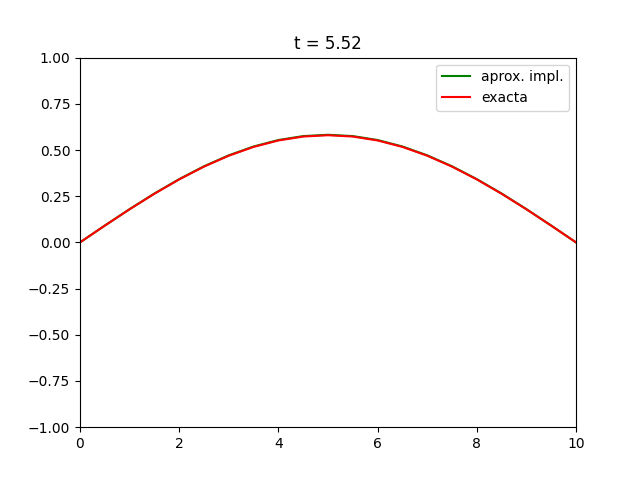
\includegraphics[scale = 0.45]{./images/Figure_1.png}
\end{subfigure}
\begin{subfigure}[b]{0.49\textwidth}
    \centering
    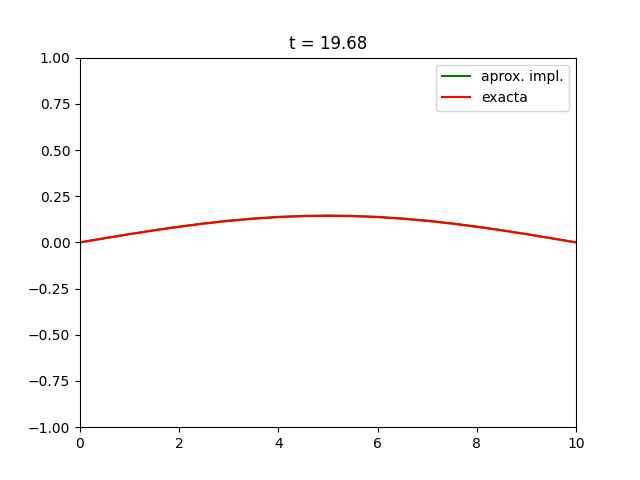
\includegraphics[scale = 0.45]{./images/Figure_2.png}
\end{subfigure}
\end{figure}
\noindent Vemos que la solución tiende a cero el tiempo tiende a infinito.

Ahora comparamos resultados con \texttt{calor\_cn\_dirichlet}, que implementa el esquema de Crank-Nicholson, y con \texttt{calor\_explicito\_dirichlet}, que implementa el esquema explícito de la práctica anterior.
\begin{center}
    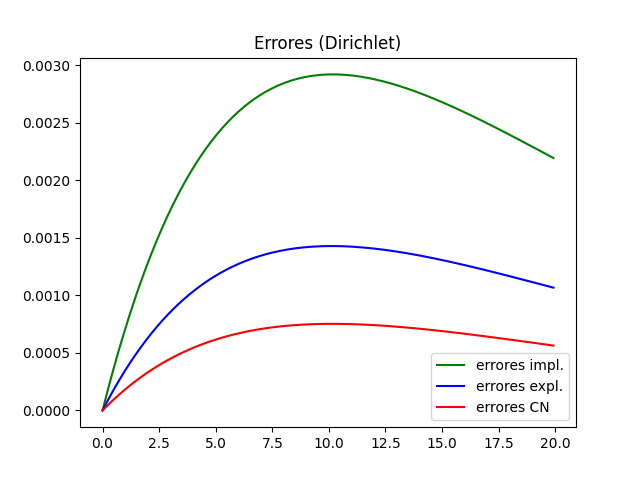
\includegraphics[scale = 0.8]{./images/Figure_3.png}
\end{center}
El tiempo de ejecución del esquema implícito es 0'010281801223754883, el del explícito, 0'010136842727661133, y el de Crank-Nicholson, 0'012889385223388672. Vemos que el esquema de Crank-Nicholson es el que comete menor error, y el esquema explícito es el más rápido. La principal desventaja del esquema explícito es que la condición CFL restringe la elección de $\Delta x$ y $\Delta t$.

Supongamos que las condiciones de contorno son de Neumann, $N_L$ a la izquierda y $N_R$ a la derecha. Supongamos también que la ecuación tiene un término fuente $F$. Como hay condiciones de Neumann, el sistema a resolver tiene $N$ ecuaciones y $N$ incógnitas. El esquema implícito es $AU^n = B^n$, donde
\[A = \left(\begin{array}{ccccc}
    1+2s & -2s & \cdots & 0 & 0 \\
    -s & 1+2s & \cdots & 0 & 0 \\
    \vdots & \vdots & \ddots & \vdots & \vdots \\
    0 & 0 & \cdots & 1+2s & -s \\
    0 & 0 & \cdots & -2s & 1+2s
\end{array}\right), \qquad U^n = \left(\begin{array}{c}
    u_0^{n+1} \\
    u_1^{n+1} \\
    \vdots \\
    u_{N-2}^{n+1} \\
    u_{N-1}^{n+1}
\end{array}\right),\]
\[B^n = \left(\begin{array}{c}
    u_0^n -2s\Delta x N_L(t_{n+1}) \\
    u_1^n \\
    \vdots \\
    u_{N-2}^n \\
    u_{N-1}^n +2s\Delta x N_R(t_{n+1}) \\
\end{array}\right)+\Delta t\left(\begin{array}{c}
    F_0^{n+1} \\
    F_1^{n+1} \\
    \vdots \\
    F_{N-2}^{n+1} \\
    F_{N-1}^{n+1} \\
\end{array}\right),\]
\normalsize
siendo $s = \frac{k\Delta t}{\Delta x^2}$ y $F_i^{n+1} = F(x_i,t_{n+1})$. El de Crank-Nicholson tiene la misma matriz de coeficientes, y el término independiente sería
\small
\[B^n = \left(\begin{array}{c}
    (1-2s)u_0^n + 2su_1^n - 2s\Delta xN_L(t_n)-2s\Delta xN_L(t_{n+1}) \\
    (1-2s)u_1^n + su_0^n + su_2^n \\
    \vdots \\
    (1-2s)u_{N-2}^n + su_{N-3}^n + su_{N-1}^n  \\
    (1-2s)u_{N-1}^n + 2su_{N-2}^n + 2s\Delta xN_R(t_n) + 2s\Delta xN_R(t_{n+1}) 
\end{array}\right)+\frac{\Delta t}{2}\left(\begin{array}{c}
    F_0^{n+1}+F_0^{n} \\
    F_1^{n+1}+F_1^{n} \\
    \vdots \\
    F_{N-2}^{n+1}+F_{N-2}^{n} \\
    F_{N-1}^{n+1}+F_{N-1}^{n} \\
\end{array}\right),\]
\normalsize
con $s = \frac{k\Delta t}{2\Delta x^2}$. 

Para terminar, comparamos los resultados de las funciones \texttt{calor\_implicito\_neumann}, \texttt{calor\_explicito\_neumann} y \texttt{calor\_cn\_neumann}.
\begin{center}
    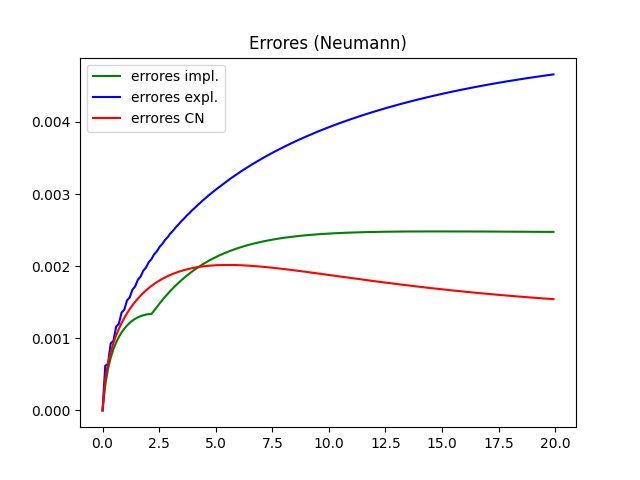
\includegraphics[scale = 0.8]{./images/Figure_4.png}
\end{center}
Ahora es el esquema explícito el que comete mayor error. El tiempo de ejecución del esquema implícito es 0'0102386474609375, el del explícito es 0'01095890998840332, y el de Crank-Nicholson es 0'01751565933227539.
\end{document}